
%----------------------------------------------------------------------------------------%
% START LaTeX preamble

% define document type, font and paper size
% \documentclass[11pt,a4paper,landscape]{slides}
\documentclass[11pt,a4paper]{slides}

%----------------------------------------------------------------------------------------%
% IMPORT LaTeX packages

\usepackage{inputenc}
\usepackage[ngerman, english]{babel}
\usepackage{csquotes}
\usepackage{amsmath}
\usepackage{amssymb}
\usepackage{amsfonts}
\usepackage{graphicx}
\usepackage{wrapfig}
\usepackage[margin=1.25in]{geometry}
\usepackage{pdfpages}
\usepackage{listings}
\usepackage{setspace}
\usepackage{systeme}
\usepackage{mdframed}
\usepackage{mmacells}
\usepackage{titling}
\usepackage{afterpage}

%----------------------------------------------------------------------------------------%
% SET user defined commands

\newcommand{\mathsym}[1]{{}}
\newcommand{\unicode}[1]{{}}
\newcommand\blankpage{%
    \null
    \thispagestyle{empty}%
    \addtocounter{page}{-1}%
    \newpage}

%----------------------------------------------------------------------------------------%
% IMPORT LaTeX packages to manange bibliography

% MLA, APA, or IEEE? - https://www.overleaf.com/learn/latex/Biblatex_citation_styles
\usepackage[style=apa]{biblatex}
\addbibresource{bibliography.bib}

%----------------------------------------------------------------------------------------%
% DEFINE header values

% define the cover page values
\title
{
    Mathematical Physical Modelling - Homework 04\\
    Differential Vector Calculus
}
\author
{
    Antonio Osamu Katagiri Tanaka    (A01212611)\\
    Diego Sebastián Ceciliano Franco (A01373414)\\
    Katya Michelle Aguilar Pérez     (A01750272)\\
}
\date{\today}
\predate{\centering}
\postdate{\vfill\hfill\emph
{
    Paper trail and process evidence are at the end of this document.
}
\hfill}

%----------------------------------------------------------------------------------------%
% USER-DEFINED commands

% Keywords command
\providecommand{\keywords}[1]
{
    \\
    \\
    \small
    \textbf{\textit{Keywords:}} #1
}

%----------------------------------------------------------------------------------------%

\begin{document}

%----------------------------------------------------------------------------------------%
% DEFINE listings setup

\lstset{basicstyle=\footnotesize\ttfamily,breaklines=true}
\lstset{numbers=left, numberstyle=\tiny, stepnumber=1, numbersep=10pt}

%----------------------------------------------------------------------------------------%
% CREATE the 1st page (cover page)

%\maketitle

%----------------------------------------------------------------------------------------%
% DEFINE the abstract text & keywords

%\begin{abstract}
%    \emph
%    {
%        Lorem ipsum dolor sit amet, consectetur adipiscing elit, sed do eiusmod tempor incididunt ut labore et dolore magna aliqua. Ut enim ad minim veniam, quis nostrud exercitation ullamco laboris nisi ut aliquip ex ea commodo consequat. Duis aute irure dolor in reprehenderit in voluptate velit esse cillum dolore eu fugiat nulla pariatur. Excepteur sint occaecat cupidatat non proident, sunt in culpa qui officia deserunt mollit anim id est laborum.
%    }
%    \keywords{Lorem, ipsum, dolor, sit, amet}
%\end{abstract}

%----------------------------------------------------------------------------------------%
\clearpage

%----------------------------------------------------------------------------------------%
% CREATE a table of contents in a new page

%\tableofcontents
%\clearpage

%----------------------------------------------------------------------------------------%
% CREATE a list of figures and a list of tables in a new page

%\listoffigures
%\listoftables
%\lstlistoflistings
%\clearpage

%----------------------------------------------------------------------------------------%
% DOCUMENT body starts here

%\section{Problemas de Eigenvalores}
%
%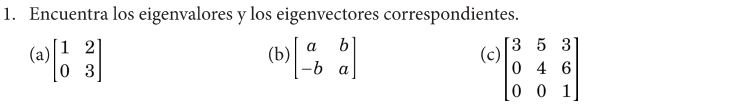
\includegraphics[width=1\textwidth]{./img/Capture1.png}
%
%\begin{mmaCell}[]{Print}
%{\normalsize Eigen-values for (a)}:
%
%\mmaSub{\(\pmb{\lambda}\)}{1}=3
%\mmaSub{\(\pmb{\lambda}\)}{2}=1
%\end{mmaCell}
%
%\begin{mmaCell}[]{Print}
%{\normalsize Eigen-vectors for (a)}:
%
%for \(\pmb{\lambda}\)=3
%\end{mmaCell}
%
%\begin{mmaCell}[verbatimenv]{Print}
%x=t\(\begin{bmatrix}
%1 \\
%1
%\end{bmatrix}\)
%\end{mmaCell}
%
%\begin{mmaCell}[]{Print}
%for \(\pmb{\lambda}\)=1
%\end{mmaCell}
%
%\begin{mmaCell}[verbatimenv]{Print}
%x=t\(\begin{bmatrix}
%1 \\
%0
%\end{bmatrix}\)
%\end{mmaCell}
%
%\begin{mmaCell}[]{Input}
%(* Verification of (a) using Mathematica's functions *)
%Eigensystem[\{\{1,2\},\{0,3\}\}];
%MatrixForm[%]
%\end{mmaCell}
%
%\begin{mmaCell}[form=MatrixForm]{Output}
%(3     1
%\{1,1\} \{1,0\})
%
%\end{mmaCell}
%
%\clearpage
%
%%----------------------------------------------------------------------------------------%
%\section{Transformaciones Lineales y Eigenvalores}
%
%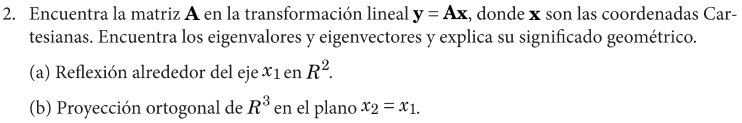
\includegraphics[width=1\textwidth]{./img/Capture2.png}
%
%\clearpage
%
%%----------------------------------------------------------------------------------------%
%\section{Aplicaciones: Deformaciones Elásticas}
%
%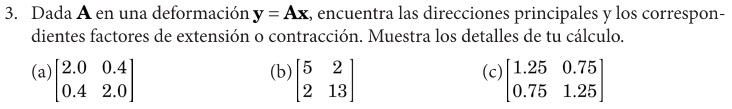
\includegraphics[width=1\textwidth]{./img/Capture3.png}
%
%\clearpage
%
%%----------------------------------------------------------------------------------------%
%\section{Aplicaciones: Modelos de Población}
%
%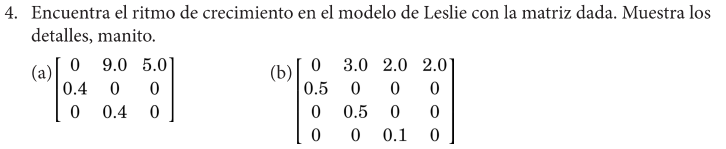
\includegraphics[width=1\textwidth]{./img/Capture4.png}
%
%\clearpage

%----------------------------------------------------------------------------------------%
%Append lectures
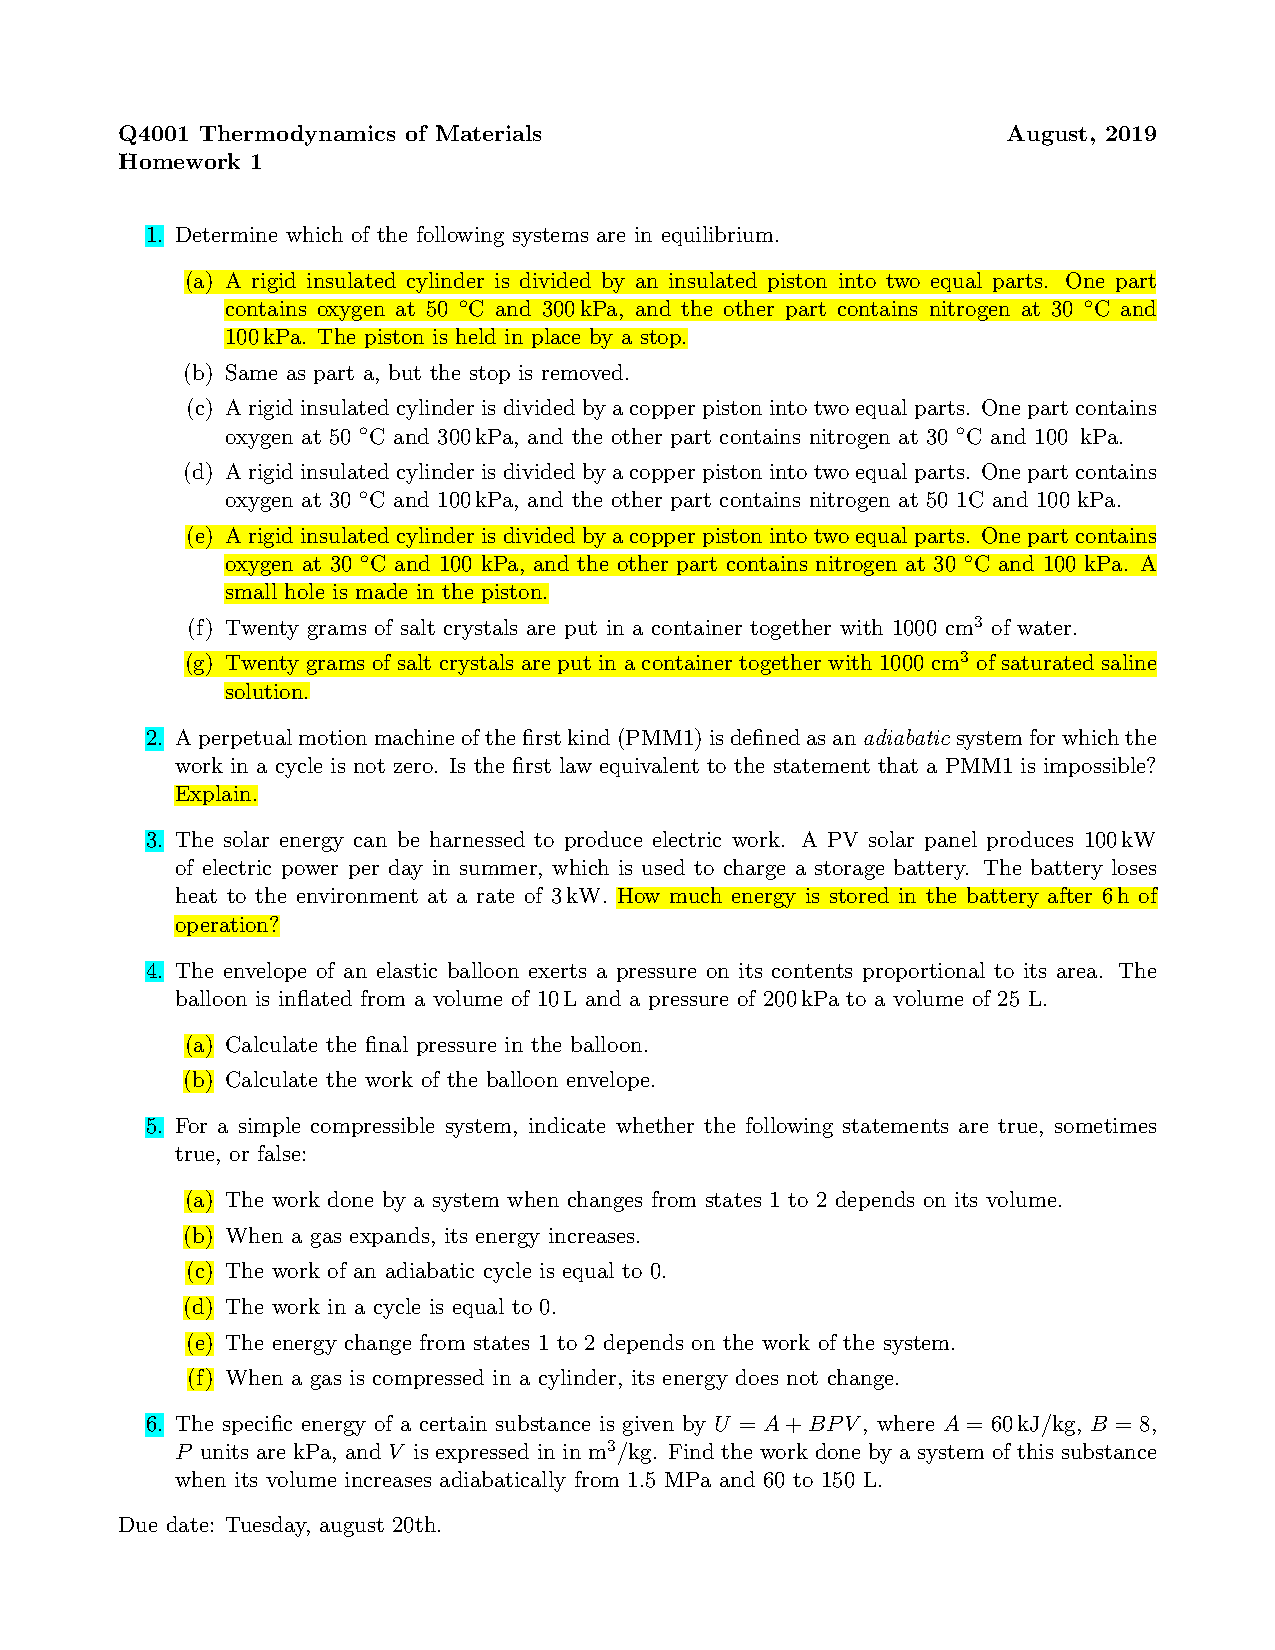
\includepdf[page=-]{./_thermo_Hwk1}
\includepdf[page=-]{./_thermo_Hwk1_paperTrail}

\clearpage

%----------------------------------------------------------------------------------------%

\end{document}

%----------------------------------------------------------------------------------------%
